%!TEX program = xelatex

\documentclass[compress]{beamer}
%--------------------------------------------------------------------------
% Common packages
%--------------------------------------------------------------------------
\usepackage[english]{babel}
\usepackage{pgfpages} % required for notes on second screen
\usepackage{graphicx}
\usepackage{subfigure}
\usepackage{multicol}
\usepackage{multirow}
\def\block(#1,#2)#3{\multicolumn{#2}{c}{\multirow{#1}{*}{$ #3 $}}}

\usepackage{fontspec}

\usepackage{tabularx,ragged2e}
\usepackage{booktabs}

\usepackage{setspace}

%--------------------------------------------------------------------------
% Load theme
%--------------------------------------------------------------------------
\usetheme{hri}

\usepackage{dtklogos} % must be loaded after theme
\usepackage{tikz}
\usetikzlibrary{arrows,shapes,snakes,calc,mindmap,backgrounds,positioning,svg.path}

\graphicspath{{figs/}}

\newcount\colveccount
\newcommand*\colvec[1]{
        \global\colveccount#1
        \begin{bmatrix}
        \colvecnext
}
\def\colvecnext#1{
        #1
        \global\advance\colveccount-1
        \ifnum\colveccount>0
                \\
                \expandafter\colvecnext
        \else
                \end{bmatrix}
        \fi
}

\tikzset{box/.style={
            draw, 
            fill=blue!20,
            fill opacity=0.8,
            thick,
            inner sep=0pt,
            minimum size=1cm,
            transform shape
        },
        finalbox/.style={
            draw, 
            fill=orange,
            fill opacity=0.8,
            thick,
            inner sep=0pt,
            minimum size=1cm,
            transform shape
        },
        dot/.style={
            draw,
            circle,
            fill=red!20,
            inner sep=0pt,
            minimum size=1cm,
            transform shape
        },
        axis/.style={
            thick,
            gray,
            font=\small},
        every to/.style={
            >=latex,
            dashed,
            thick
        }
    }



%--------------------------------------------------------------------------
% General presentation settings
%--------------------------------------------------------------------------
\title{Introduction à l'infographie 3D}
\subtitle{CS211 -- Introduction à l'informatique visuelle}
\date{24 février 2015}
\author{Séverin Lemaignan}
\institute{Computer-Human Interaction\\for Learning and Instruction {\Medium
EPFL}}

%--------------------------------------------------------------------------
% Notes settings
%--------------------------------------------------------------------------
%\setbeameroption{show notes on second screen}
%\setbeameroption{hide notes}

\begin{document}

\maketitle

%%%%%%%%%%%%%%%%%%%%%%%%%%%%%%%%%%%%%%%%%%%%%%%%%%%%%%%%%%%%%%%%%%%%%%%%%%%%%%%

\section{We are all Pixar}

\imageframe{sintel.png}

\imageframe{sintel-opengl-textures.png}
\imageframe{sintel-opengl.png}
\imageframe{sintel-wireframe.png}
\imageframe{sintel-vertices.png}

\begin{frame}{}

    Pipeline: from a cube in 3D to rasterization
\end{frame}

%%%%%%%%%%%%%%%%%%%%%%%%%%%%%%%%%%%%%%%%%%%%%%%%%%%%%%%%%%%%%%%%%%%%%%%%%%%%%%%
%%%%%%%%%%%%%%%%%%%%%%%%%%%%%%%%%%%%%%%%%%%%%%%%%%%%%%%%%%%%%%%%%%%%%%%%%%%%%%%

\section{La boite à outil mathématique}

\begin{frame}{Point, vecteur}
\end{frame}
\begin{frame}{Produit vectoriel}

    $ \vec{a} \times \vec{b} = \colvec{3}{a_x}{a_y}{a_z} \times
    \colvec{3}{b_x}{b_y}{b_z} = \colvec{3}{a_yb_z - a_zb_y}{a_zb_x -
    a_xb_z}{a_xb_y - a_yb_x} $
    
    \input{sketches/normal_vector.tex}
\end{frame}

%%%%%%%%%%%%%%%%%%%%%%%%%%%%%%%%%%%%%%%%%%%%%%%%%%%%%%%%%%%%%%%%%%%%%%%%%%%%%%%

\section[Transformations]{Transformations linéaires}

\begin{frame}{Transformation linéaire}
\Large
\[
    T(x) = Ax
\]
\end{frame}

\begin{frame}{Expression matricielle}

Quelle matrice $\mathbf{A}$ représente la transformation linéaire $T(x)$
(par exemple, l'homothétie $T(x) = 5x$)?

\uncover<2->{
Dans la base canonique $\{\vec{e_1}, \vec{e_2}, \ldots, \vec{e_n}\}$,

$\mathbf{A} = \begin{bmatrix} T( \vec e_1 ) & T( \vec e_2 ) & \cdots & T( \vec
e_n ) \end{bmatrix}$
}

\uncover<3->{

    Dans le plan,

$T( \vec{x} ) = 5 \vec{x} = 5 \mathbf{I} \vec{x} = \begin{bmatrix} 5 && 0 \\ 0
                                                                     && 5
\end{bmatrix} \vec{x}$
}
\end{frame}

\begin{frame}{Matrices de rotation}

\[
    \left\{
        \begin{array}{lr}
            x' = x \cos \theta + y \sin\theta \\
            y' =  -x \sin \theta + y \cos\theta
        \end{array}
    \right.
\]

    \uncover<2->{
\[
    \begin{bmatrix} x' \\ y' \end{bmatrix} = \begin{bmatrix} \cos \theta &
    \sin\theta \\ -\sin \theta & \cos \theta \end{bmatrix} \begin{bmatrix} x \\ y
    \end{bmatrix}
\]
}
\only<3>{
    \centering
    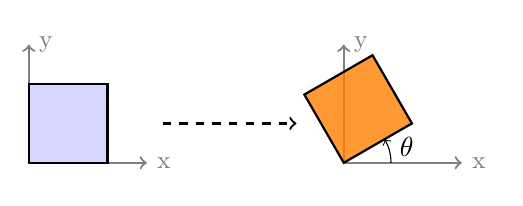
\begin{tikzpicture}
        \draw[axis,->] (0,0) -- (1.5,0) node[right] {x};
        \draw[axis,->] (0,0) -- (0,1.5) node[right] {y};

        \draw[axis,->] (4,0) -- (5.5,0) node[right] {x};
        \draw[axis,->] (4,0) -- (4,1.5) node[right] {y};

        \draw[dashed, thick, ->] (1.7,0.5) -- (3.4,0.5);

        \node[box] at (0.5,0.5) (base) {};
        \node[finalbox,rotate around={30:(-0.5,-0.5)}] at (4.5,0.5) (transformed) {};

        \draw[solid,->] (4.6,0) arc(0:30:0.6);
        \node at (4.8,0.2) {$\theta$};

    \end{tikzpicture}

}
\only<4>{
    Dans l'espace, une rotation $\theta$ autour de l'axe définit par le vecteur
    $(l, m, n)$:
    \[
        \left[\begin{smallmatrix}
            ll(1-\cos \theta)+\cos\theta & ml(1-\cos\theta)-n\sin\theta &
            nl(1-\cos\theta)+m\sin\theta\\
            lm(1-\cos\theta)+n\sin\theta & mm(1-\cos\theta)+\cos\theta &
            nm(1-\cos\theta)-l\sin\theta \\
            ln(1-\cos\theta)-m\sin\theta & mn(1-\cos\theta)+l\sin\theta &
            nn(1-\cos\theta)+\cos\theta
    \end{smallmatrix}\right]
    \]
}

\end{frame}

\begin{frame}{Cisaillement (shearing)}
    \begin{multicols}{2}

\[
\begin{bmatrix} x' \\ y' \end{bmatrix} = \begin{bmatrix} 1 & k \\ 0 & 1
\end{bmatrix} \begin{bmatrix} x \\ y \end{bmatrix}
\]
    \centering
    
\begin{tikzpicture}
       \node[box] at (0,0) (base) {};
        \node[finalbox,cm={1,0,1,1,(0,0)}] at (3,0) (transformed) {};
        \draw[dashed, thick, ->] (1,0) -- (2,0);
    \end{tikzpicture}

    \end{multicols}

    \begin{multicols}{2}

\[
\begin{bmatrix} x' \\ y' \end{bmatrix} = \begin{bmatrix} 1 & 0 \\ k & 1
\end{bmatrix} \begin{bmatrix} x \\ y \end{bmatrix}
\]
    \centering
    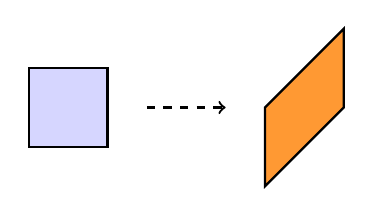
\begin{tikzpicture}
        \node[box] at (0,0) {};
        \node[finalbox,cm={1,1,0,1,(0,0)}] at (3,0) {};
        \draw[dashed, thick, ->] (1,0) -- (2,0);
    \end{tikzpicture}

    \end{multicols}


\end{frame}

\begin{frame}{}

Quelle transformation représente la matrice ci-dessous ?

\[
\begin{bmatrix} x' \\ y' \end{bmatrix} = \begin{bmatrix} 1 & 0 \\ 0 & 0
\end{bmatrix} \begin{bmatrix} x \\ y \end{bmatrix}
\only<1>{
\]
}
\only<2>{
= \begin{bmatrix} x \\ 0 \end{bmatrix} 
\]
}

\end{frame}

\begin{frame}{}

    Représenter les transformations sous forme matricielle est particulièrement
    efficace (opérations ne requiérant que des multiplications et des additions,
    vectorisation via SSE).

    \uncover<2->{
    \LARGE
    Mais pour les transformations \textbf{non linéaires}? (...comme les translations)
    }

\end{frame}


%%%%%%%%%%%%%%%%%%%%%%%%%%%%%%%%%%%%%%%%%%%%%%%%%%%%%%%%%%%%%%%%%%%%%%%%%%%%%%%

\section{Coordonnées homogènes}



\begin{frame}{Intuition}
    \only<1-4>{
    \[
    \begin{bmatrix} x' \\ y' \end{bmatrix} = \begin{bmatrix} 1 & k \\ 0 & 1
    \end{bmatrix} \begin{bmatrix} x \\ y \end{bmatrix}
    \]
    }
    \only<1>{
    \centering
    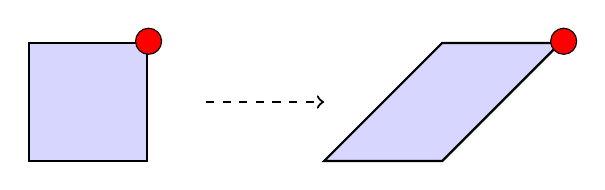
\begin{tikzpicture}[scale=1.5]
        \node[box] at (0,0) (base) {};
        \node[box,cm={1,0,1,1,(0,0)}] at (3,0) (transformed) {};
        \draw (base.north east) node[minimum size=0.1cm,draw,circle,fill=red] {};
        \draw (transformed.north east) node[minimum size=0.1cm,draw,circle,fill=red] {};
        \draw[dashed, thick, ->] (1,0) -- (2,0);
    \end{tikzpicture}

    }
    \only<2>{
        \centering
    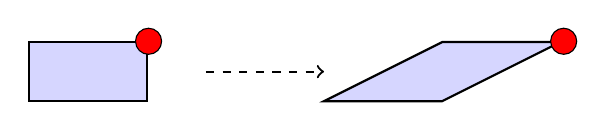
\begin{tikzpicture}[scale=1.5]
        \begin{scope}[cm={1,0,0,0.5,(0,0)}]
            \node[box] at (0,0) (base) {};
            \node[box,cm={1,0,1,1,(0,0)}] at (3,0) (transformed) {};
        \end{scope}
        \draw (base.north east) node[minimum size=0.1cm,draw,circle,fill=red] {};
        \draw (transformed.north east) node[minimum size=0.1cm,draw,circle,fill=red] {};
        \draw[dashed, thick, ->] (1,0) -- (2,0);
    \end{tikzpicture}
    }
    \only<3>{
        \centering

    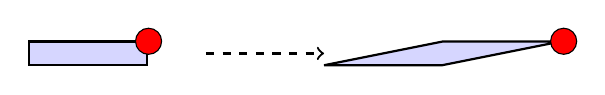
\begin{tikzpicture}[scale=1.5]
        \begin{scope}[cm={1,0,0,0.2,(0,0)}]
            \node[box] at (0,0) (base) {};
            \node[box,cm={1,0,1,1,(0,0)}] at (3,0) (transformed) {};
        \end{scope}
        \draw (base.north east) node[minimum size=0.1cm,draw,circle,fill=red] {};
        \draw (transformed.north east) node[minimum size=0.1cm,draw,circle,fill=red] {};
        \draw[dashed, thick, ->] (1,0) -- (2,0);
    \end{tikzpicture}
    
    }
    \only<4>{
        \centering

    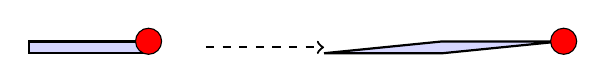
\begin{tikzpicture}[scale=1.5]
        \begin{scope}[cm={1,0,0,0.1,(0,0)}]
            \node[box] at (0,0) (base) {};
            \node[box,cm={1,0,1,1,(0,0)}] at (3,0) (transformed) {};
        \end{scope}
        \draw (base.north east) node[minimum size=0.1cm,draw,circle,fill=red] {};
        \draw (transformed.north east) node[minimum size=0.1cm,draw,circle,fill=red] {};
        \draw[dashed, thick, ->] (1,0) -- (2,0);
    \end{tikzpicture}

    }
    \only<5>{
        \centering
        \video{0.7\textwidth}{videos/affine_transformations.ogv}\\
        \vspace*{1em}
    }

    \uncover<6->{
        \textbf{Idée clé} : ajouter une dimension (\emph{coordonnée $w$}) pour linéariser les \textbf{transformations
        affines} (comme les translations) et les \textbf{transformations
        projectives} (on va y revenir).
    }
\end{frame}

\begin{frame}{}
\[
\begin{bmatrix} x' \\ y' \\ 1 \end{bmatrix} = \begin{bmatrix} 1 & 0 & t_x \\ 0
                                                                 & 1 & t_y \\ 0
                                                                 & 0 & 1
\end{bmatrix} \begin{bmatrix} x \\ y \\ 1 \end{bmatrix} = \begin{bmatrix} x +
    t_x \\ y + t_y
\\ 1 \end{bmatrix}
\]

\uncover<2-> {
    Une translation en 2D (transformation affine) peut être représentée comme un
    cisaillement en 3D (transformation linéaire).
}
\end{frame}

\begin{frame}{Espace projectif et coordonnées homogènes}

$\begin{bmatrix} x \\ y \\ w \end{bmatrix}$ représente \textbf{une} des
\textbf{coordonnées homogènes} du point $\begin{bmatrix} x \\ y \end{bmatrix}$ dans \textbf{l'espace
    projectif} $\mathbb{P}(\mathbb{R})$ associé à l'espace euclidien
        $\mathbb{R}^2$.

        \uncover<1->{
$(kx, ky, k), k \in \mathbb{R}\setminus\{0\}$ représente \textbf{l'ensemble des coordonnées homogènes} du point
$(x, y)$.
}

\uncover<2->{
Pour repasser en coordonnées euclidiennes, il suffit de diviser par la
coordonnée $w$: $\begin{bmatrix} x/w \\ y/w \\ 1 \end{bmatrix}$.
}

\end{frame}

\begin{frame}{Coordonnées homogènes (2)}
    \centering
    Si $\begin{bmatrix} x \\ y \\ 1 \end{bmatrix}$ est un point 2D, que penser
    de $\begin{bmatrix} x \\ y \\ 0 \end{bmatrix}$?

        \uncover<2->{
        \Large
            Point à l'infini\\
            ou vecteur\\
            ou direction
        }

            \uncover<3->{
                \normalsize
        L'espace projectif permet \emph{d'équiper l'espace euclidien
        avec des points à l'infini}
    }

\end{frame}

\begin{frame}{En 3D}


\only<1>{

Coordonnées homogènes: $[x, y, z, w]^\intercal$

Translations :
\[
\begin{bmatrix} x' \\ y' \\ z' \\ 1 \end{bmatrix} = \begin{bmatrix} 1 & 0 & 0 & t_x \\
                                                                    0 & 1 & 0 & t_y \\
                                                                    0 & 0 & 1 & t_z \\
                                                                    0 & 0 & 0 & 1
\end{bmatrix} \begin{bmatrix} x \\ y \\ z \\ 1 \end{bmatrix} = \begin{bmatrix} x +
    t_x \\ y + t_y \\ z + t_z \\ 1 \end{bmatrix}
\]

Rotations :

\[
\begin{bmatrix} x' \\ y' \\ z' \\ 1 \end{bmatrix} = \begin{bmatrix}
    \block(3,3){R_{3 \times 3}} & 0 \\
                 &  &  & 0 \\
                 &  &  & 0 \\
                 0 & 0  & 0 & 1
\end{bmatrix} \begin{bmatrix} x \\ y \\ z \\ 1 \end{bmatrix}
\]
}

\only<2>{
    Homothétie (isotropique si $\alpha = \beta = \gamma$, anisotropique sinon):
\[
\begin{bmatrix} x' \\ y' \\ z' \\ 1 \end{bmatrix} = \begin{bmatrix} \alpha & 0 & 0 & 0 \\
                                                                    0 & \beta & 0 & 0 \\
                                                                    0 & 0 & \gamma & 0 \\
                                                                    0 & 0 & 0 & 1
\end{bmatrix} \begin{bmatrix} x \\ y \\ z \\ 1 \end{bmatrix} = \begin{bmatrix} \alpha x \\ \beta y \\ \gamma z \\ 1 \end{bmatrix}
\]


}

\end{frame}

\section{Composition de transformations}

\begin{frame}{Composition de transformations}
    Simple multiplication de matrices !
    $\mathbf{B}(\mathbf{A} \vec{x} ) = (\mathbf{BA}) \vec{x}$

    \uncover<2->{
        Attention : la multiplication de matrices est associative, mais
        \textbf{pas commutative} en général!
        

        Rotation $\mathbf{A}$ suivie de Translation $\mathbf{B}$ $\equiv \mathbf{BA}\vec{x}$ et non
        $\mathbf{AB}\vec{x}$!

    \begin{multicols}{2}
    \centering
    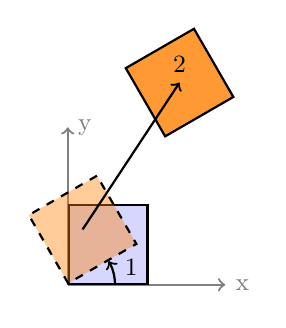
\begin{tikzpicture}[every node/.style={anchor=south west}]
        \draw[axis,->] (0,0) -- (2,0) node[right] {x};
        \draw[axis,->] (0,0) -- (0,2) node[right] {y};

        \node[box] at (0,0) (base) {};
        \begin{scope}[rotate=30]
            \node[box,dashed, fill opacity=0.4, fill=orange] at (0,0) (mid) {};
            \node[finalbox, cm={1,0,0,1,(2,1)}] at (0,0) (final) {};
        \end{scope}
        \draw[thick,->] (0.6,0) arc(0:30:0.6);
        \node at (.6,0) {\small 1};
        \draw[thick, ->] (mid.center) -- (final.center) node[above] {\small 2};


    \end{tikzpicture}
\vfill
\columnbreak
\vspace*{\fill}
    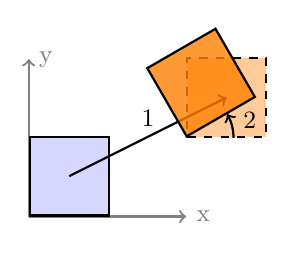
\begin{tikzpicture}[every node/.style={anchor=south west}]
        \draw[axis,->] (0,0) -- (2,0) node[right] {x};
        \draw[axis,->] (0,0) -- (0,2) node[right] {y};

        \node[box] at (0,0) (base) {};
        \begin{scope}[cm={1,0,0,1,(2,1)}]
            \node[box,dashed, fill opacity=0.4, fill=orange] at (0,0) (mid) {};
            \draw[thick, ->] (base.center) -- (mid.center) node[midway,above] {\small 1};
            \node[finalbox, rotate=30] at (0,0) (final) {};
        \end{scope}

        \draw[thick,->] (2.6,1) arc(0:30:0.6);
        \node at (2.6,1) {\small 2};

    \end{tikzpicture}


    \end{multicols}


    }
\end{frame}

\begin{frame}{Matrices de transformation généralisées}

\[
\begin{bmatrix} 1 & 0 & t_x \\
                0 & 1 & t_y \\
                0 & 0 & 1
\end{bmatrix} 
\begin{bmatrix} 
            \cos \theta  & \sin\theta & 0 \\ 
           -\sin \theta & \cos \theta & 0 \\
            0 & 0 & 1
\end{bmatrix}
\only<1>{
= ?
}
\uncover<2->{
= \begin{bmatrix} 
            \cos \theta  & \sin\theta & t_x \\ 
           -\sin \theta & \cos \theta & t_y \\
            0 & 0 & 1
\end{bmatrix}
}
\]

\uncover<3->{

\[
\begin{bmatrix} \alpha & 0 & 0 \\
                0 & \beta & 0 \\
                0 & 0 & 1
\end{bmatrix} 
\begin{bmatrix} 1 & 0 & t_x \\
                0 & 1 & t_y \\
                0 & 0 & 1
\end{bmatrix} 
\begin{bmatrix} 
            \cos \theta  & \sin\theta & 0 \\ 
           -\sin \theta & \cos \theta & 0 \\
            0 & 0 & 1
\end{bmatrix}
= \begin{bmatrix} 
            \alpha \cos \theta  & \sin\theta & t_x \\ 
           -\sin \theta & \beta \cos \theta & t_y \\
            0 & 0 & 1
\end{bmatrix}
\]

\uncover<4->{
    \centering
    \Large
    \textbf{Dans quel ordre ?}
}
}

   %\input{sketches/transformations-base.tex}

\end{frame}

\begin{frame}{En 3D}
\[
\begin{bmatrix} x' \\ y' \\ z' \\ 1 \end{bmatrix} = \begin{bmatrix}
    \block(3,3){R_{3 \times 3}} & \block(1,3){T_{1 \times 3}} \\
                 &  &  &  \\
                 &  &  &  \\
                 0 & 0  & 0 & 1
\end{bmatrix} \begin{bmatrix} x \\ y \\ z \\ 1 \end{bmatrix}
\]
\end{frame}

\begin{frame}{Scene Graph}
    \begin{center}
    \only<1>{
    \input{sketches/scene-graph.tex}
}
    \only<2->{
    \input{sketches/scene-graph-cube.tex}
}

    \uncover<3->{
        \texttt{matrixPush()}, \texttt{matrixPop()}!
    }
    \end{center}
\end{frame}
%%%%%%%%%%%%%%%%%%%%%%%%%%%%%%%%%%%%%%%%%%%%%%%%%%%%%%%%%%%%%%%%%%%%%%%%%%%%%%%

\section{Les projections}


\begin{frame}{Projection}
    \begin{center}
        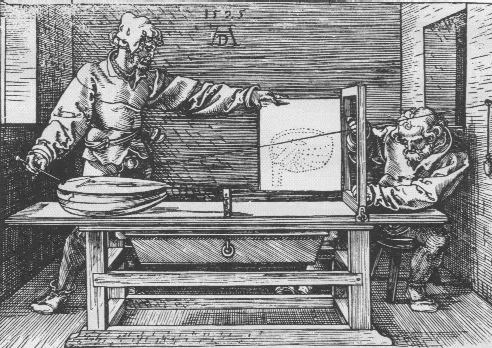
\includegraphics[width=0.8\linewidth]{durer-projection}
    \end{center}
\end{frame}

\begin{frame}{Rappel: Produit scalaire}
    \begin{center}

\[
    \vec{a} \cdot \vec{b} = \colvec{3}{a_x}{a_y}{a_z} \cdot
    \colvec{3}{b_x}{b_y}{b_z} = \| \vec{a} \| \| \vec{b} \| cos \theta = a_x b_x + a_y b_y + a_z b_z 
\]

    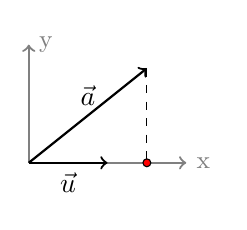
\begin{tikzpicture}
        \draw[axis,->] (0,0) -- (2,0) node[right] {x};
        \draw[axis,->] (0,0) -- (0,1.5) node[right] {y};

        \draw[thick,->] (0,0) -- (1.5,1.2) node[above,midway]{$\vec{a}$};
        \draw[thick,->] (0,0) -- (1,0) node[below,midway]{$\vec{u}$};
        \draw[thin, dashed] (1.5,1.2) -- (1.5,0) {};

        \draw (1.5,0) node[inner sep=0,minimum size=0.1cm,draw,circle,fill=red] {};

    \end{tikzpicture}

    Projection de $\vec{a}$ sur $\vec{u}$ : $(\vec(a) \cdot \vec{u}) \vec{u}$

    \uncover<2>{
        Que se passe-t'il pour des vecteurs orthogonaux ?
    }
    \end{center}
\end{frame}

\begin{frame}{Projection}
    \centering
    \input{sketches/projection.tex}
\end{frame}

\begin{frame}{}

\begin{center}
    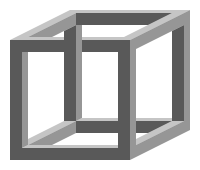
\includegraphics[width=0.8\linewidth]{impossible_cube}
\end{center}

\end{frame}

%%%%%%%%%%%%%%%%%%%%%%%%%%%%%%%%%%%%%%%%%%%%%%%%%%%%%%%%%%%%%%%%%%%%%%%%%%%%%%%

\section{Rendu 3D}


%%%%%%%%%%%%%%%%%%%%%%%%%%%%%%%%%%%%%%%%%%%%%%%%%%%%%%%%%%%%%%%%%%%%%%%%%%%%%%%

\section{Pour aller plus loin}

\begin{frame}{Lumières et ombres}
\end{frame}

\begin{frame}{Raytracing}
\end{frame}

%%%%%%%%%%%%%%%%%%%%%%%%%%%%%%%%%%%%%%%%%%%%%%%%%%%%%%%%%%%%%%%%%%%%%%%%%%%%%%%

\section{Dans la vraie vie}

\begin{frame}{}
    TDB: video game screenshot
    -> need to be fast and to approximate stuff
\end{frame}

\begin{frame}{}
    OpenGL (and co)
\end{frame}


\begin{frame}{Exemple de question}
\end{frame}

\end{document}






